% !TeX root = main.tex

\subsection{Why relative homology?}

The primary tool used in the TCC that we will apply to the analysis of scalar fields is relative persistent homology.
Relative homology provides a powerful representation of a bounded domain that is particularly suited to verifying coverage of a sensor network.
Let $\D$ be a bounded domain with boundary $\B\subset\D$.
For illustrative purposes assume $\D$ is a connected, compact subset of the euclidean plane $\R^2$ so that certain properties of the relative homology of the pair $(\D, \B)$ are known.
Namely, there is exactly one equivalence class in $\hom_2(\D, \B)$, as illustrated in Fig.~\ref{fig:balloons1}.
We can think of the quotient as an identification of points in the boundary, illustrated by wrapping the planar domain around a single point in $\R^3$.
As the domain is compact this creates a single void corresponding to the one generator in $\hom_2(\D, \B)$.

\figblock{%
\begin{figure}[htbp]
\centering
    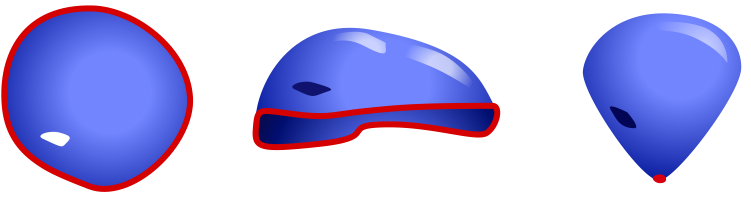
\includegraphics[scale=0.5]{figures/balloons2.png}
    \caption{If there is a gap in the domain that is not a part of the boundary then $\beta_2 = \rank~ \hom_2(\D, \B) = 0$ as there is no void.}
    \label{fig:balloons2}
\end{figure}}

Now suppose our network $P$ covers the domain at some scale $\delta > 0$ such that there are no gaps (1-cycles) in $P^\delta$.
The subset $Q = \B^\delta \cap P$ of points within distance $\delta$ of $\B$ gives us a pair $(P^\delta, Q^\delta)$.
We can verify that the set $P$ covers some subset of the domain by the same process.
A gap in coverage can be through of as ``popping the balloon'' in the sense that, if we wrap the set $P^\delta$ around $Q^\delta$ we would have no void---the gap provides a hole through which the ``air'' can escape, as illustrated in Fig.~\ref{fig:balloons2}.

\subsection{Why short filtrations?}

As we are interested in the coordinate-free setting we will compute the homology of our network using a pair of Rips complexes $\rips_\delta(P, Q) = (\rips_\delta(P),\rips_\delta(Q))$ included into a pair of Rips complexes $\rips_\gamma(P, Q)$.
The reason for this is twofold.

\paragraph{Rips-\v Cech interleaving}

First, the homology of the \v Cech complex can be recovered from this inclusion via the Rips-\v Cech interleaving
\[ \rips_\delta(P, Q) \subseteq \cech_\delta(P, Q)\subseteq \rips_{2\delta}(P,Q).\]
By the nerve theorem this pair of \v Cech complexes is homotopy equivalent to the pair of offsets $(P^\delta, Q^\delta)$ as desired.

\paragraph{Fake cycles}
Second, consider a situation in which $P^\delta$ covers $\D$ but there is an additional cycle in $\hom_1(Q^\delta)$ that does not reflect a feature of $\hom_1(\B)$.
In this case there is some point $x\in\D$ surrounded by this cycle that is covered by a point in $P\setminus Q$ but not $Q$.
The result is a non-zero element in $\hom_2(P^\delta, Q^\delta)$ that reflects the void containing this point and not the void corresponding to an element of $\hom_2(\D,\B)$, leading us to a false positive.
Fortunately, this situation is resolved by once again looking at the inclusion $(P^\delta, Q^\delta)\hookrightarrow (P^\gamma, Q^\gamma)$ as any such ``spurious'' cycles are killed for sufficiently large $\gamma > 0$.
This inclusion is contained in the inclusion of Rips complexes $\rips_\delta(P, Q)\hookrightarrow\rips_{2\gamma}(P, Q)$ as follows
\[ \rips_\delta(P, Q) \hookrightarrow \cech_\delta(P,Q)\hookrightarrow\cech_\gamma(P,Q)\hookrightarrow\rips_{2\gamma}(P, Q). \]

\begin{figure}[htbp]
\centering
    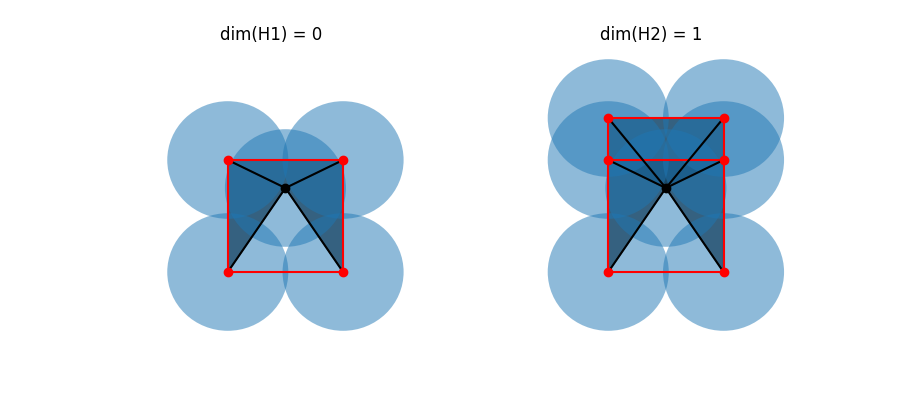
\includegraphics[scale=0.7]{figures/counter.png}
\end{figure}

% In order to verify coverage we therefore need an element in $\hom_2(P^\delta, Q^\delta)$ that \emph{persists} until $\hom_2(P^\gamma, Q^\gamma)$.
%
% An element in $\hom_1(P^\delta\hookrightarrow P^\gamma)$ that does not correspond to an element of $\hom_1(\B)$ surely indicates a gap in coverage.
% However,
%
% Any element of $\hom_1(P^\delta)$ that does not correspond to an element of $\hom_1(\D)$ indicates a gap in coverage of the \emph{whole} domain $\D$.
% These are the elements which ``kill'' the void we expect in $\hom_2(P^\delta, Q^\delta)$.
%
% Any element of $\hom_1(Q^\delta)$ that is trivial in $\hom_1(P^\delta)$ must be the boundary of an element of $\hom_2(P^\delta, Q^\delta)$ by exactness.
%
% Because $\B$ is the topological boundary of $\D$ any element of $\hom_1(\B)$ that is trivial in $\hom_1(\D)$ must be the boundary of an element
%

\subsection{Why $\D\setminus\B^{2\delta}$ (TODO)?}

Suppose there exists a non-trivial element $[x]$ in $\im~\hom_2((P^\delta, Q^\delta)\hookrightarrow (P^\gamma, Q^\gamma))$.
Clearly $[x]\notin\hom_2(P^\delta)$ and $[x]\notin\hom_2(P^\gamma)$ so there must be chains in $C_2(P^\delta)$ and $C_2(P^\gamma)$ with boundaries in $C_1(Q^\delta)$ and $C_1(Q^\gamma)$.
If these chains correspond to those in $C_2(\D)$ and $C_1(\B)$ we have a good representation of our domain.
However, boundaries

Suppose there is a non-trivial element $[x]$ in $\hom_2(P^\delta, Q^\delta)$.
Because we are working in $\R^2$ we know that $[x]\notin \hom_2(P^\delta)$ so there must exist a chain in $C_2(P^\delta)$ with its boundary in $C_1(Q^\delta)$.
If this chain corresponds to the maximal chain in $C_2(\D)$ with boundary equal to the topological boundary, an element of $C_1(\B)$, we have no issue.
However, consider a cycle in $C_1(P^\delta)$ that corresponds to a gap in coverage

% The elements of $\im~\hom_2((P^\delta, Q^\delta)\hookrightarrow (P^\gamma, Q^\gamma))$ are those in $\hom_2(P^\delta, Q^\delta)$ which \emph{persist} until $\hom_2(P^\gamma, Q^\gamma)$.
% Any additional elements in $\hom_2(P^\gamma, Q^\gamma)$ that are not in $\hom_2(P^\delta, Q^\delta)$ will not be found in the inclusion.


% As we are interested in the coordinate-free setting we cannot compute the homology of the pair of \emph{offsets} $(P^\delta, Q^\delta)$ directly.
%
%
% Two fundamental issues arise in this process.
% First, we cannot compute the homology of the pair of \emph{offsets} $(P^\delta, Q^\delta)$ directly.
% Given precise coordinates of the sensors we could use the pair of \v Cech complexes $\cech_\delta(P, Q) = (\cech_\delta(P), \cech_\delta(Q))$ which is homotopy equivalent by the nerve theorem.
% However, we are interested in the coordinate-free case in which we have only pairwise proximity data between sensors.
% Second,
%
% Therefore, we must use the interleaving of the Rips and \v Cech to
%
%
% However, we are
% Even by using the nerve lemma to replace the pair of offsets with the pair of \v Cech
% Recall that the nerve lemma states that the
% Although we can compute the homology of the pair of \v Cech complexes, denoted , with the precise coordinates of our sensors we
% % % Given such a pair $(P, Q)$ let $\rips_\delta(P, Q)$ denote the pair of complexes $(\rips_\delta(P), \rips_\delta(Q))$ throughout.
% % Our goal now is to check if the relative homology $\hom_2(P^\delta, Q^\delta)$ of the pair $(P^\delta, Q^\delta)$ reflects that of our domain $(\D, \B)$.
% % A gap in coverage can be thought of as
%
% % Now suppose our network $P$ covers the domain at some scale $\delta > 0$ such that there are no gaps (1-cycles) in $\rips_\delta(P)$.
% % The subset $Q = \{p\in P\mid \ball_\delta(p)\cap\B\neq\emptyset\}$ of points within distance $\delta$ of $\B$ induces a subcomplex $\rips_\delta(Q)$ of $\rips_\delta(P)$.
% % Given such a pair $(P, Q)$ let $\rips_\delta(P, Q)$ denote the pair of complexes $(\rips_\delta(P), \rips_\delta(Q))$ throughout.
% % Under our assumptions, the relative homology $H_2(\rips_\delta(P, Q))$ should reflect that of the domain.
% % A gap in coverage can be thought of as ``popping the balloon'' in the sense that, if we wrap the simplices of $\rips_\delta(P)$ around those in $\rips_\delta(Q)$ we would have no void---the gap provides a hole through which the ``air'' can escape, as illustrated in Fig.~\ref{fig:balloons2}.

\subsection{What do we have? How can we use it?}

A collection of sensors can be verified as covering a domain if
\begin{enumerate}
    \item[a.] the boundary of the domain is adequately covered,
    \item[b.] the balloon has not been ``punctured.''
\end{enumerate}
Condition (b) relies on condition (a) in order to provide a topological condition that is necessary but not sufficient.
Given (a) we can confirm coverage by checking if the balloon has been punctured simply by checking the dimension of the top-dimensional relative homology of the sample.
Adequate coverage of the boundary can be broken into two parts.
First, we require that the sampled boundary is in some sense simple in order to ensure our condition cannot produce false positives.
This is achieved by using what we refer to as \emph{short-filtrations}: applying one step of persistence in order to de-noise the data.
By testing our network at two scales we can ensure no spurious features are present in the boundary which may contribute to false positives.
We also note that these short-filtrations are employed in the analysis of scalar fields as well.

Secondly, we require that the so-called ``sampled boundary'' surrounds the interior of the domain.
Otherwise, we may cover the domain but see what looks like a punctured ball as the ball when in fact the ball was never formed.
In the TCC this situation is not handled explicitly.
Instead it is stated as a condition for coverage that is necessary but not sufficient.
That is, it can verify \emph{coverage} without false positives but may produce false negatives.
In fact, the TCC tests a more specific problem: whether we have a reliable representation of the boundary \emph{and} a reliable representation of the interior.

Given this observation we considered how best two use \emph{all} the information given by the TCC in a way that re-uses the machinery used to compute it.
We therefore consider consider the relative persistent homology of a domain modulo a sublevel-set.
That is, we re-cast the TCC for a domain defined as a domain surrounded by sub-level set of a function on that domain in order to ensure that a given sample can adequately approximate the relative homology of the domain modulo a sub-level set.
We then modify the analysis of scalar fields in order to give an approximation of the \emph{relative} persistent homology of a sample.
Finally, we consider classes of functions which satisfy the assumptions made.
Namely, we consider functions with multiple sub-level sets which may serve as a boundary for this procedure and show how they can be integrated to give a more robust signature for the function.
